% !Mode:: "TeX:UTF-8"	% read in as utf8 file.

\section{Constant Strain Triangle}
\subsection{Nodal displacements}
The triangular membrane element is considered to lie in the $ xy $ plane of a local $ xy $ coordinate system as shown in Figure \ref{fig: CST_element}. The nodes are arranged as $ 1,2 $ and $ 3 $ in anti-clockwise. Each node includes 2 degrees of freedom . The displacement components can be expressed as:

\begin{equation}
\mathbf{q}^e = \left\lbrace
\begin{array}{c}
u_1 \\
v_1 \\
u_2 \\
v_2 \\
u_3 \\
v_3
\end{array} \right \rbrace
\end{equation}

\begin{figure}[h!]
	\centering
	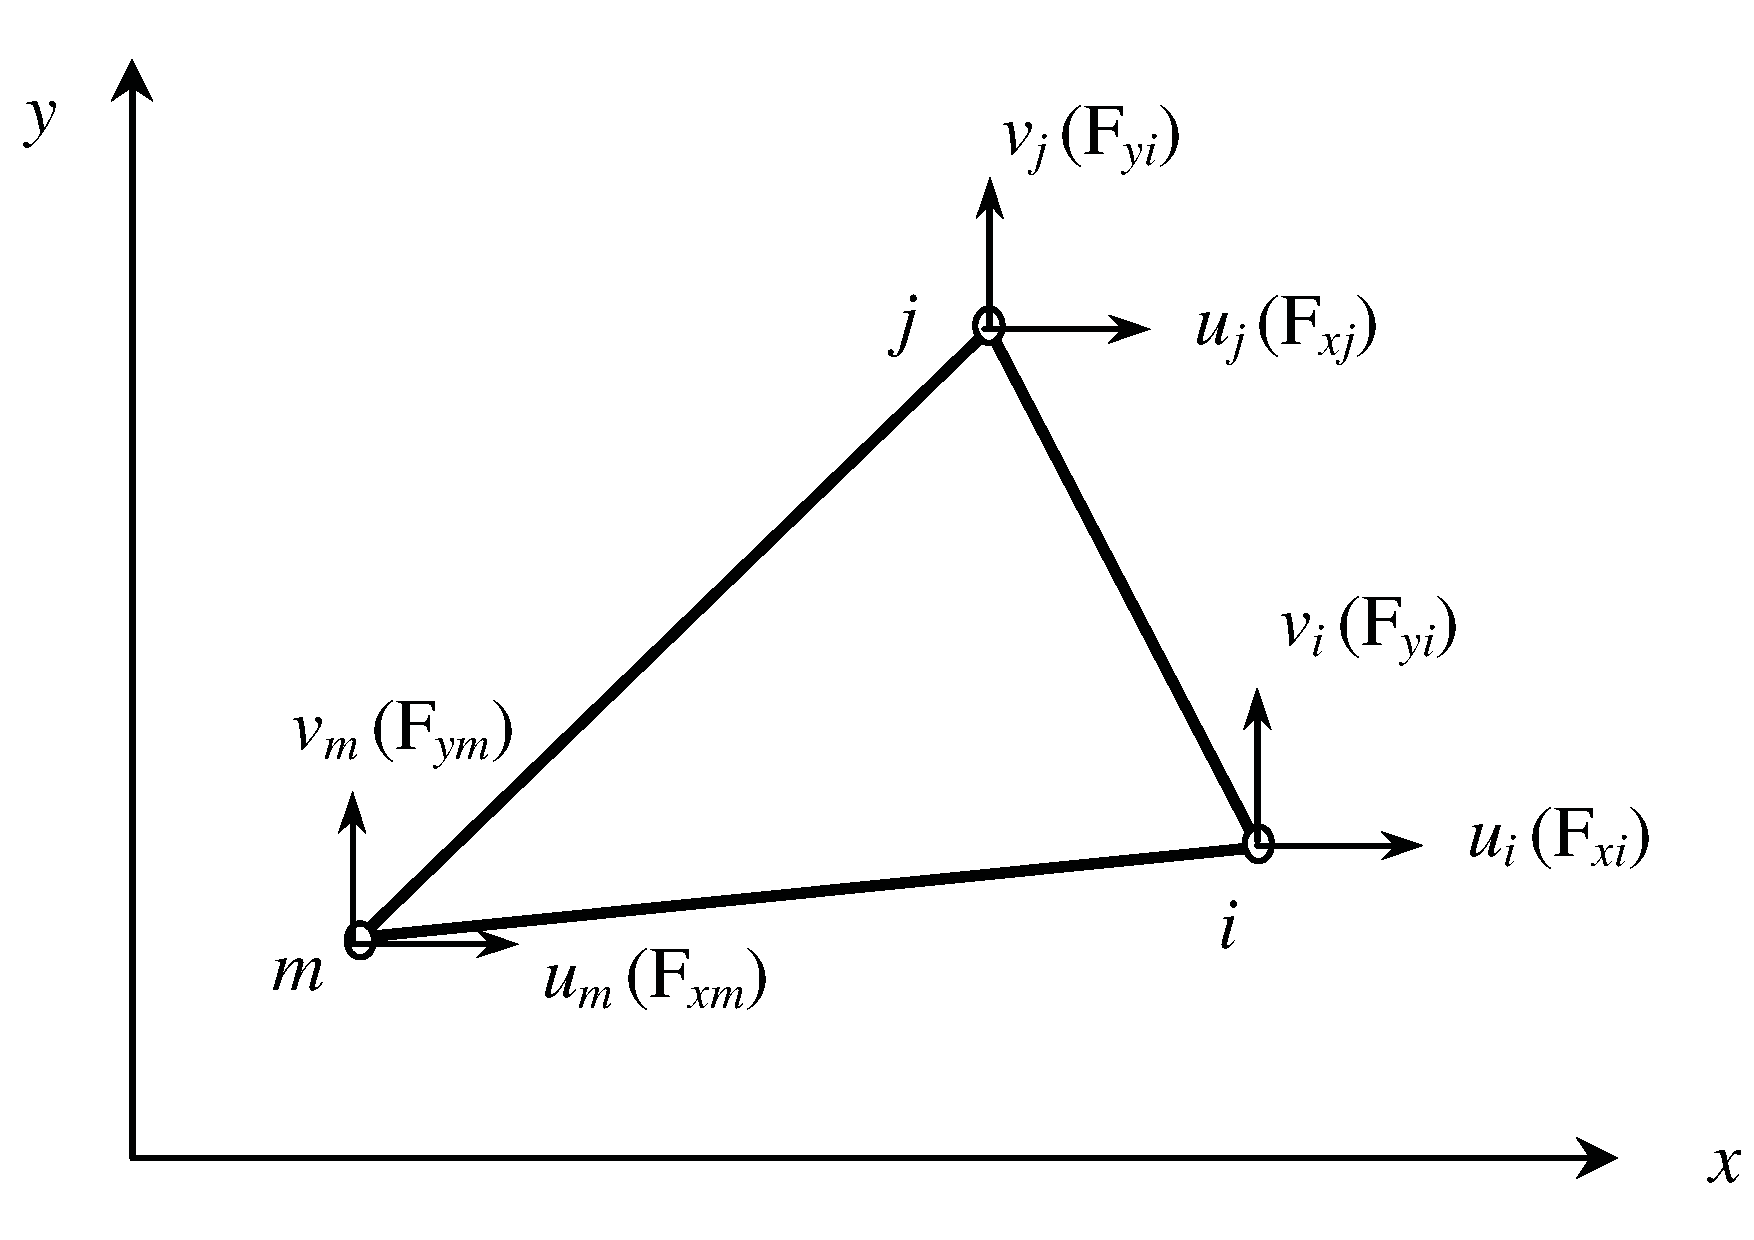
\includegraphics[width=0.5\linewidth]{figures/CST_element}
	\caption{Triangular membrane element}
	\label{fig: CST_element}
\end{figure}

\subsection{Shape functions}
By assuming a linear displacement variation inside the element and introducing a set of area coordinates, the displacement model can be expressed as:

\begin{equation} \label{eq: CST_displacement_model}
\begin{split}
u &= a_1 + a_2 x + a_3 y \\
v &= a_4 + a_5 x + a_6 y
\end{split}
\end{equation}

By considering the displacements $ u_i $ and $ v_i $ as the local degrees of freedom of node $ 1,2,3 $, the constants $ a_1, \cdots, a_6 $ can be evaluated. Thus, by using the conditions

\begin{align*}
	u_1 &= a_1 + a_2 x_1 + a_3 y_1 & v_1 &= a_4 + a_5 x_1 + a_6 y_1 \\
	u_2 &= a_1 + a_2 x_2 + a_3 y_2 & v_2 &= a_4 + a_5 x_2 + a_6 y_2 \\
	u_3 &= a_1 + a_2 x_3 + a_3 y_3 & v_3 &= a_4 + a_5 x_3 + a_6 y_3
\end{align*}

We can express the constants $ a_1, \cdots, a_6 $ in terms of the nodal degrees of freedom:

\begin{align*}
	a_1 &= \frac{1}{2\Delta} 
	\begin{vmatrix}
		u_1 & x_1 & y_1 \\ 
		u_2 & x_2 & y_2 \\ 
		u_3 & x_3 & y_3
	\end{vmatrix} & a_2 &= \frac{1}{2\Delta} 
	\begin{vmatrix}
		1 & u_1 & y_1 \\ 
		1 & u_2 & y_2 \\ 
		1 & u_3 & y_3
	\end{vmatrix} & a_3 &= \frac{1}{2\Delta} 
	\begin{vmatrix}
		1 & x_1 & u_1 \\ 
		1 & x_2 & u_2 \\ 
		1 & x_3 & u_3
	\end{vmatrix} 
\end{align*}

Where 

\begin{equation*}
2\Delta = \begin{vmatrix}
	1 & x_1 & y_1 \\ 
	1 & x_2 & y_2 \\ 
	1 & x_3 & y_3
\end{vmatrix}
\end{equation*}

This leads to the displacement model:
\begin{equation*}
	\mathbf{N} \mathbf{q}^e = \begin{bmatrix}
	N_1 & 0 & N_2 & 0 & N_3 & 0 \\ 
	0 & N_1 & 0 & N_2 & 0 & N_3
\end{bmatrix} \left\lbrace\begin{array}{c}
u_1 \\ 
v_1 \\ 
u_2 \\ 
v_2 \\ 
u_3 \\ 
v_3
\end{array} \right\rbrace
\end{equation*}

\begin{align*}
	a_1 &= x_2 y_3 - x_3 y_2 & a_2 &= x_3 y_1 - x_1 y_3 & a_3 &= x_1 y_2 - x_2 y_1 \\
	b_1 &= y_2 - y_3 & b_2 &= y_3 - y_1 & b_3 &= y_1 - y_2 \\
	c_1 &= x_3 - x_2 & c_2 &= x_1 - x_3 & c_3 &= x_2 - x_1 \\
	N_1 &= \frac{( a_1 + b_1 x + c_1 y)}{2\Delta} & N_2 &= \frac{( a_2 + b_2 x + c_2 y)}{2\Delta} & N_3 &= \frac{( a_3 + b_3 x + c_3 y)}{2\Delta}
\end{align*}

\subsection{Element Strain}
By using the relations:

\begin{equation}
\mathbf{\varepsilon} = \left\lbrace \begin{array}{c}
\varepsilon_{xx} \\ 
\varepsilon_{yy} \\ 
\varepsilon_{xy}
\end{array} \right\rbrace = \left\lbrace \begin{array}{c}
\frac{\partial u}{\partial x} \\ 
\frac{\partial v}{\partial y} \\ 
\frac{\partial u}{\partial y}+\frac{\partial v}{\partial x}
\end{array}  \right\rbrace 
\end{equation}

the components of strain can be expressed in terms of nodal displacements as:

\begin{equation}
\mathbf{\varepsilon} = \mathbf{B} \mathbf{q}^e
\end{equation}

where

\begin{equation}\label{eq: CST_strain_disp_matrix}
\mathbf{B} = \frac{1}{2\Delta} \begin{bmatrix}
b_1 & 0 & b_2 & 0 & b_3 & 0 \\ 
0 & c_1 & 0 & c_2 & 0 & c_3 \\ 
c_1 & b_1 & c_2 & b_2 & c_3 & b_3
\end{bmatrix} 
\end{equation}

\subsection{Element stress}
The stress-strain relations are given by:

\begin{equation}\label{eq: CST_stress}
\mathbf{\sigma} = \mathbf{D} \mathbf{\varepsilon}
\end{equation}

where

\begin{equation}
\mathbf{\sigma} = \left\lbrace \begin{array}{c}
\sigma_{xx} \\ 
\sigma_{yy} \\ 
\sigma_{xy}
\end{array}  \right\rbrace
\end{equation}

and

\begin{equation}\label{eq: CST_stress_strain_matrix}
\mathbf{D} = \frac{E}{1-\nu^2} \begin{bmatrix}
1 & \nu & 0 \\ 
\nu & 1 & 0 \\ 
0 & 0 & \frac{1-\nu}{2}
\end{bmatrix} 
\end{equation}

\subsection{Element stiffness}
the stiffness matrix of the element $ \mathbf{K}_e $ can be found by using:

\begin{equation}\label{eq: CST_stiffness_matrix_definition}
\mathbf{K}_e=\iiint_\Omega \mathbf{B}^T \mathbf{DB} d\Omega = \iint_\Delta \mathbf{B}^T \mathbf{DB} h d\Delta
\end{equation}

where $ \Omega $ denotes the volume of the element. If the plate thickness is taken as a constant $ h $, the evaluation of the integral in eq \ref{eq: CST_stiffness_matrix_definition} presents no difficult since the elements of the matrices $ \mathbf{B} $ and $ \mathbf{D} $ are all constants (not functions of $ x $ and $ y $). Hence, Eq \ref{eq: CST_stiffness_matrix_definition} can be rewritten as:

\begin{equation}\label{eq: CST_stiffness_matrix}
\mathbf{K}_e = \mathbf{B}^T \mathbf{DB} h \iint_\Delta   d\Delta =  h\Delta \mathbf{B}^T \mathbf{DB}
\end{equation}
